\chapter{Introduction}\label{ch1}

Depth camera technologies have gotten a lot of attention lately. The key reason behind its substantial popularity growth and technological advancements is the fact that a lot of computer vision applications rely on its 3D sensing capabilities. As the demand for Machine Learning (ML) systems grow, we observe a rapid growth of the technologies using 3D sensing systems across different technology areas, be it a consumer electronics, self-driving cars or drones. The one such market which has gotten noticeably better and cheaper lately is the consumer depth camera market. Embedded into the latest generation of smartphones, depth camera modules found its way to scale of consumers. Standalone depth cameras also got better, cheaper and smaller while maintaining its qualitative advantages. While the former are designed to enhance overall image quality, stability and introduce industry's first dedicated sensor based Augmented Reality (AR) features inside the mobile operating system, the latter are designed to deal with a wide range of computationally heavy and accuracy focused applications. Such applications include object detection, motion tracking, face scanning, object reconstruction, etc. \bigskip 

In this thesis, we focus on the 3D reconstruction of the human face. A dense 3D face reconstruction from a single 2D image is a long-standing and widely researched topic in computer vision. Approaches include, model based probabilistic approaches\cite{Romdhani3DM, Schoenborn2017, 10.1007/978-3-642-40602-7_11} or nowadays the more popular convolution neural networks (CNN)\cite{Guo_2019, tu2019joint}. The aim of this thesis is to incorporate consumer depth camera capabilities into the existing model based 3D face reconstruction pipeline hereafter referred to as a face fitting pipeline using 3D Morphable Model (3DMM)\cite{Blanz:1999:MMS:311535.311556, Romdhani3DM}. We also attempt to replicate and potentially improve the result of the original 2D face fitting pipeline \cite{Schoenborn2017} as well as augmented depth fitting \cite{betschard2016} pipeline, which proved to improve the original approach. The original 2D fitting approach was performing the reconstruction based solely on a single image, while its improved version was utilizing an additional depth image information. Our main goal is to design and implement a stable client-server based system which robustly and efficiently takes care of all the sensitive details of both the image capturing procedure and later face fitting pipeline. In addition to that, we will investigate the possibility to speed up the fitting process so that the final pipeline could be used for live demos and could seamlessly be integrated into the existing Scalismo Face Morpher web service (Figure \ref{f1.1}). 

\begin{figure}
    \centering
    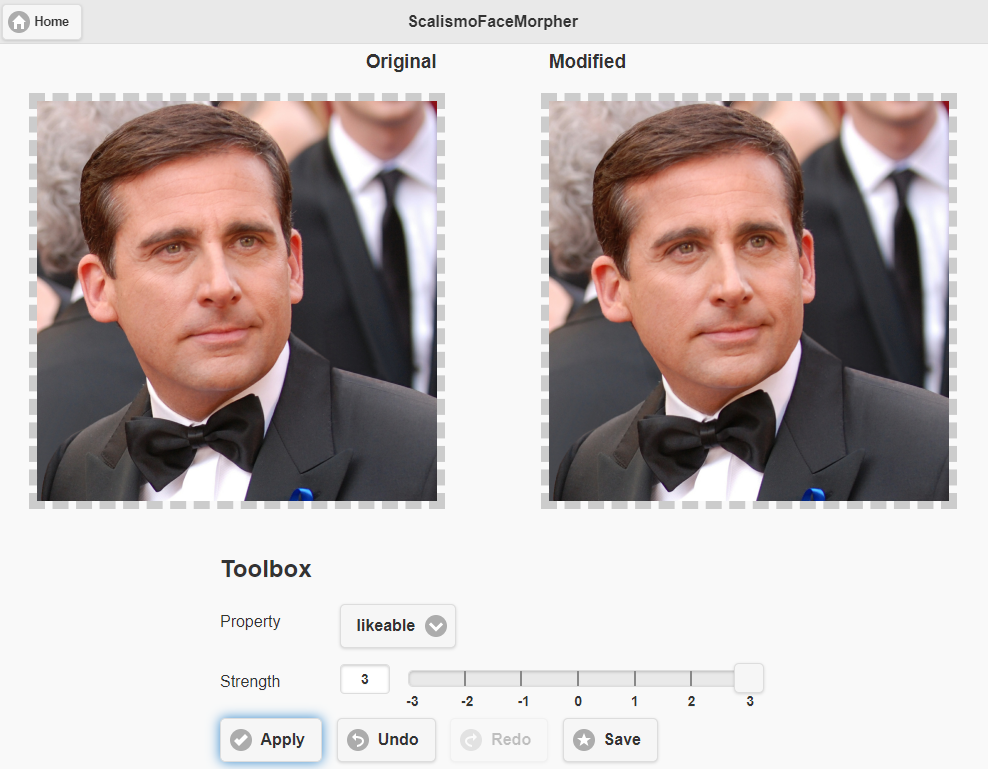
\includegraphics[width=\textwidth]{Figures/site.PNG}
    \caption{Scalismo Face Morpher website — \url{https://face-morpher.scalismo.org}.}
    \label{f1.1}
\end{figure} 

\section{Motivation \& Previous Work} 
Reconstructing a 3D face from a single 2D image is a challenging task. The major issue the fitting process has to overcome is to efficiently recover the 3D shape information and overall appearance of the face in the image. The appearance of the face in the 3DMM environment is being controlled by a set of model parameters that control faces pose, shape, expression, color, and illumination. Face fitting, therefore, is a pipeline that takes a 2D color image with a human face in it (hereafter referred to as a target image) as an input and attempts to find the best possible set of parameters mentioned above by using Analysis-by-Synthesis paradigm\cite{Schoenborn2014,10.1007/978-3-642-40602-7_11}. The key idea of the Analysis-by-Synthesis is to generate a synthetic face image which is close to an observed target image. By doing so, the fitting process fits 3DMM face model to the face appearing in the image such that, the fitted model instance (hereafter referred to as the best fit or simply fit) represents the target face as accurately as possible. Thus, the result of the face fitting pipeline is a synthetic face matching to the target face in the image and replicating all the important characteristics of it.\bigskip

The complexity of inferring a face appearance from a single 2D image using the Analysis-by-Synthesis approach was investigated by Sch{\"o}nborn et al. \cite{Schoenborn2014, Schoenborn2017, 10.1007/978-3-642-40602-7_11}. Considering the fact that the project was solely relying on a single 2D image that only holds information about the color intensities, quite good results were achieved. However, since the amount of information that can be utilized from a 2D image is limited, the authors proposed an idea of improving the standard 2D face fitting pipeline by combining the RGB data with the depth information obtained from a dedicated depth camera. Betschard et al. \cite{betschard2016} investigated this idea by using Intel® RealSense™ F200 depth camera and demonstrated that it is possible to improve the reconstruction quality of the initial method by up to 35\%. The authors of the latter research also proposed an idea of further improving the pipeline by relying on an additional point cloud information, which we thoroughly investigate in this thesis, and at the same time attempt to improve the efficiency and robustness of the fitting pipeline as a whole.\bigskip

The main difference between a 3D depth camera and a normal 2D image capturing camera is that a depth camera instead of taking just a 2D RGB-color image also has an ability to produce a point cloud of the scene. A point cloud is a set of data points produced by the camera based on the combination of information obtained from the depth sensors and cameras' intrinsic parameters. Each point is located in the 3D coordinate system representing a direct mapping of pixels in the color image. This means that the number of points in a point cloud object directly correlates to the number of pixels in the corresponding color image. Therefore, each point in a point cloud represents an $(x, y, z)$ tuple (coordinates) with the coordinate $(0, 0, 0)$ referring to the center of the physical camera sensor\cite{rs-projection}, the $z$ axes in this tuple is called depth (or $z$-Buffer). It corresponds to a distance, measured from the camera to each corresponding pixel in the 2D color image. It is clear that having $(x, y, z)$ coordinates will represent the pixel location in 3D coordinate space more accurately than having just a $z$-Buffer which was used by \cite{betschard2016}; and obviously, this would give us significantly more information (especially, regarding the shape information of the face), than standard fitting can extract from a 2D image. Therefore, the performance, efficiency, and quality of majority applications, that only make use of the information extracted from a single 2D image could be potentially improved by employing a 3D depth information obtained from the depth camera. \bigskip

\begin{figure}
    \centering
    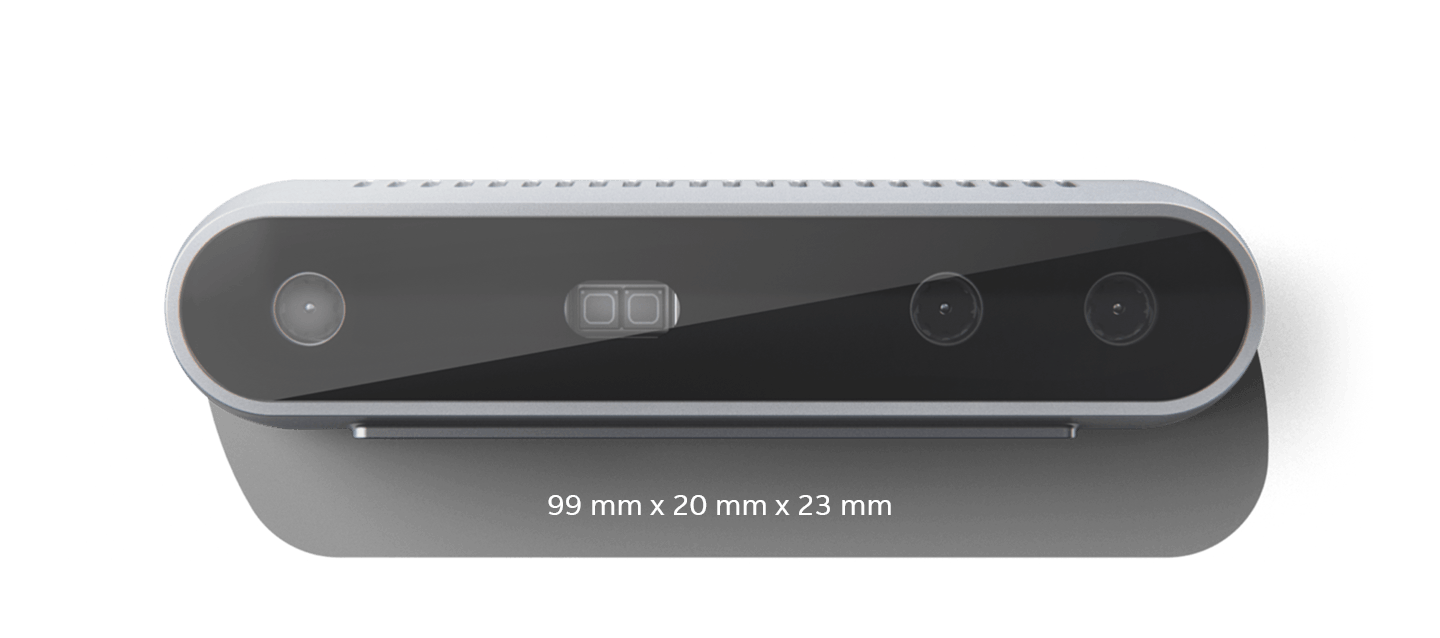
\includegraphics[width=\textwidth]{Figures/stereo_DT_d415_front-crop1a-1.png}
    \caption{Intel® RealSense™ D415 camera equipped with an array of sensors (left to right) depth sensor 1, infrared (IR) projector, depth sensor 2, color sensor. Source: Intel}
    \label{f1.2}
\end{figure}

We will be leveraging the latest generation Intel® RealSense™ D400 series depth camera shown in Figure \ref{f1.2} to obtain all necessary data for the fitting pipeline - including an RGB color image, a mesh constructed from point cloud, and a set of facial landmarks. The camera retails under 200CHF and it is one of the best affordable 3D depth cameras currently available on the market. Designed specificity for 3D scanning, portable D415 offers a good accuracy (Z-Accuracy $\leq$2\% also known as the absolute error)\footnote{The accuracy depends on the camera calibration procedure.} and dedicated powerful computer vision processor for on-the-fly calculations.


\section{Contributions}
In this work, we have made the following contributions. 1) We have implemented a new fitting pipeline, which in addition to color image also integrates a 3D depth information into the fitting process. We propose a new modular approach for solving this problem which utilizes point cloud information that is being captured from the camera.  2) We have implemented a client-server based modular system, which splits camera configuration, data acquisition, shape fitting, and color fitting procedures from each other. Thanks to its modularity, the system introduces additional flexibility and ease of use for any potential future applications. 3) We have successfully integrated our system into already existing Scaismo Face Morpher service (Figure \ref{f1.1}), which provides the possibility to use our modules for demo purposes. 4) We evaluated our proposed implementation based on a dataset that consists of a series of sample shots that we have made using our data capturing procedure, and present results at the end of the thesis. 
% We propose a new modular approach for solving the problem of human face reconstruction based on a single image with additional point cloud information obtained from the depth camera. Splitting data acquisition, shape fitting, and color fitting procedures from each other our system introduces additional flexibility and ease of use for any potential future projects. Besides the complete client-server based system, our main contributions include the data acquisition and the shape fitting procedures.

\section{Thesis Structure}
We structure this thesis as follows. The details of all the above mentioned procedures combined with background material necessary to follow the flow of events and concepts we employ throughout this thesis will be elaborated in Chapter \ref{ch2}. We introduce the model that we will be using for our application, as well as, describe the idea and implementation of a novel fitting pipeline. We also give a quick overview of depth camera technologies and how they work. Including how pixel-to-point and point-to-pixel de-projection is performed based on a pinhole camera model.  We then proceed with describing the methods (Chapter \ref{ch3}) we used to implement a reliable system. Chapter starts with describing our module based system, including the description of each of its key modules and components. We first introduce our camera of choice, its calibration procedure, and parameter configuration together with a software development kit (SDK) that allows us to seamlessly communicate with the camera and utilize its depth sensing capabilities. We further introduce a client-server based architecture that successfully delivers the data from the camera to the Scala client. The data client receives from the server is then being used to perform our proposed shape fitting pipeline and later slightly modified color fitting pipeline. Chapter \ref{ch4} contains the results and the evaluation of our method and its performance comparison to a novel fitting method. We also provide intermediate comparison results between the shape and color fitting modules to ensure that the final output is within the limits of our desired result and it actually improves previous achievements. An example result of our proposed method can be seen in Figure \ref{f1.3}. 

\begin{figure}
    \centering
    \begin{minipage}{0.49\textwidth}
        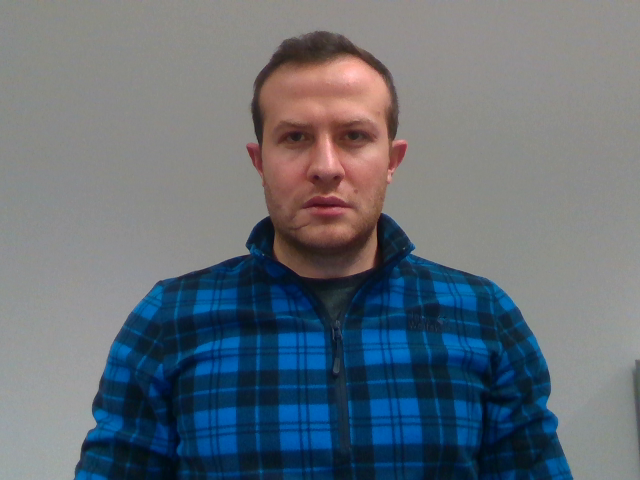
\includegraphics[width=0.999\textwidth]{Figures/dataset/target/1.png}
    \end{minipage}
    \begin{minipage}{0.49\textwidth}
        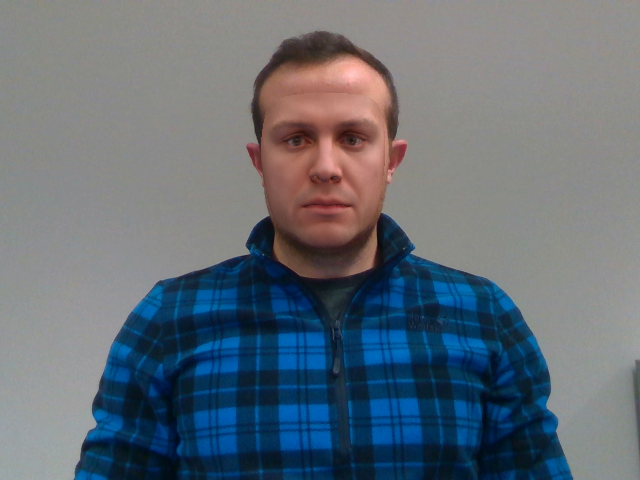
\includegraphics[width=0.999\textwidth]{Figures/dataset/our/1blended.png}
    \end{minipage}
    \caption{Example fitting result with target image (left) and synthetic fit produced by our method (right).}
    \label{f1.3}
\end{figure}

In Chapter \ref{ch5} we summarize our work and provide conclusions, followed by Chapter \ref{ch6} where we propose a couple of potential improvements that can be done to further improve the stability and performance of our system. 

